\documentclass[]{article}
\usepackage[utf8]{inputenc}
\usepackage[ngerman]{babel}
\usepackage[T1]{fontenc}
\usepackage{%
	ngerman,
	ae,
	times,  %% hier kann man die Schriftart einstellen
	graphicx,
	url,
	scrlayer-scrpage,
	lastpage,
	mathtools,
	geometry,
	multicol,
	cancel,
	xcolor,
	nicematrix,
	xfrac,
	tikz,
	pgfplots,
	amsmath,
	colortbl,
	centernot,
	dsfont,
	textgreek,
	icomma,
	pdfpages,
	kvmap}
\usepackage[thinlines]{easybmat}
\usetikzlibrary{datavisualization}
\usetikzlibrary{datavisualization.formats.functions}
\usetikzlibrary{intersections}
\pgfplotsset{compat=1.17}
\newcommand{\del}[1]{\cancel{~#1~}}
\NiceMatrixOptions{ last-col,code-for-last-col = \color{blue}\scriptstyle,light-syntax}
\newlength\dlf
\newcommand\alignedhighlight[3]{
  % #1 = color
  % #2 = before alignment
  % #3 = after alignment
  &
  \begingroup
  \settowidth\dlf{$\displaystyle #2$}
  \addtolength\dlf{\fboxsep+\fboxrule}
  \hspace{-\dlf}
  \fcolorbox{#1}{#1}{$\displaystyle #2 #3$}
  \endgroup
}
\newcommand{\reference}[1]{ \text{\small{\textcolor{blue}{(#1)}}} }

\newcommand{\topic}{Grundlagen Technische Informatik}
\newcommand{\subtopic}{Versuch 2}
\newcommand{\authors}{Kleingruppe A2}

%Head and Footnotes
\setlength{\headheight}{2.1\baselineskip} %baselineskip = minimum distance bbetween the bottom of one line to another.
\geometry{bottom = 3cm}
\setlength{\headsep}{\baselineskip}
\ihead[\topic\hrule]{\topic\hrule}
\chead[\subtopic\\~]{\subtopic\\~}
\ohead[\authors\\~]{\authors\\~}
\ifoot[~]{~}
\cfoot[~]{~}
\ofoot[Seite \thepage~von \pageref{LastPage}]{Seite \thepage~von \pageref{LastPage}}

%Paragraph spacings
\setlength{\parindent}{0em} %em = with of an 'M'
\setlength{\parskip}{1ex} %ex = height of an 'x'


\newcommand{\V}{\lor}
\newcommand{\A}{\land}
\newcommand{\T}[1]{\overline{#1}}
\newcommand{\eq}{\Leftrightarrow}
\newcommand{\rarr}{\Rightarrow}
\newcommand{\red}[1]{\textcolor{red}{#1}}

\newcommand{\unit}[1]{\text{#1}}
\newcommand{\fracunit}[2]{\frac{\unit{#1}}{\unit{#2}}}
\newcommand{\textsq}[1]{\ensuremath{\text{#1}^2}}
\newcommand{\textpow}[2]{\ensuremath{\text{#1}^{#2}}}
\newcommand{\tdot}{\ensuremath{\cdot}}


\begin{document}
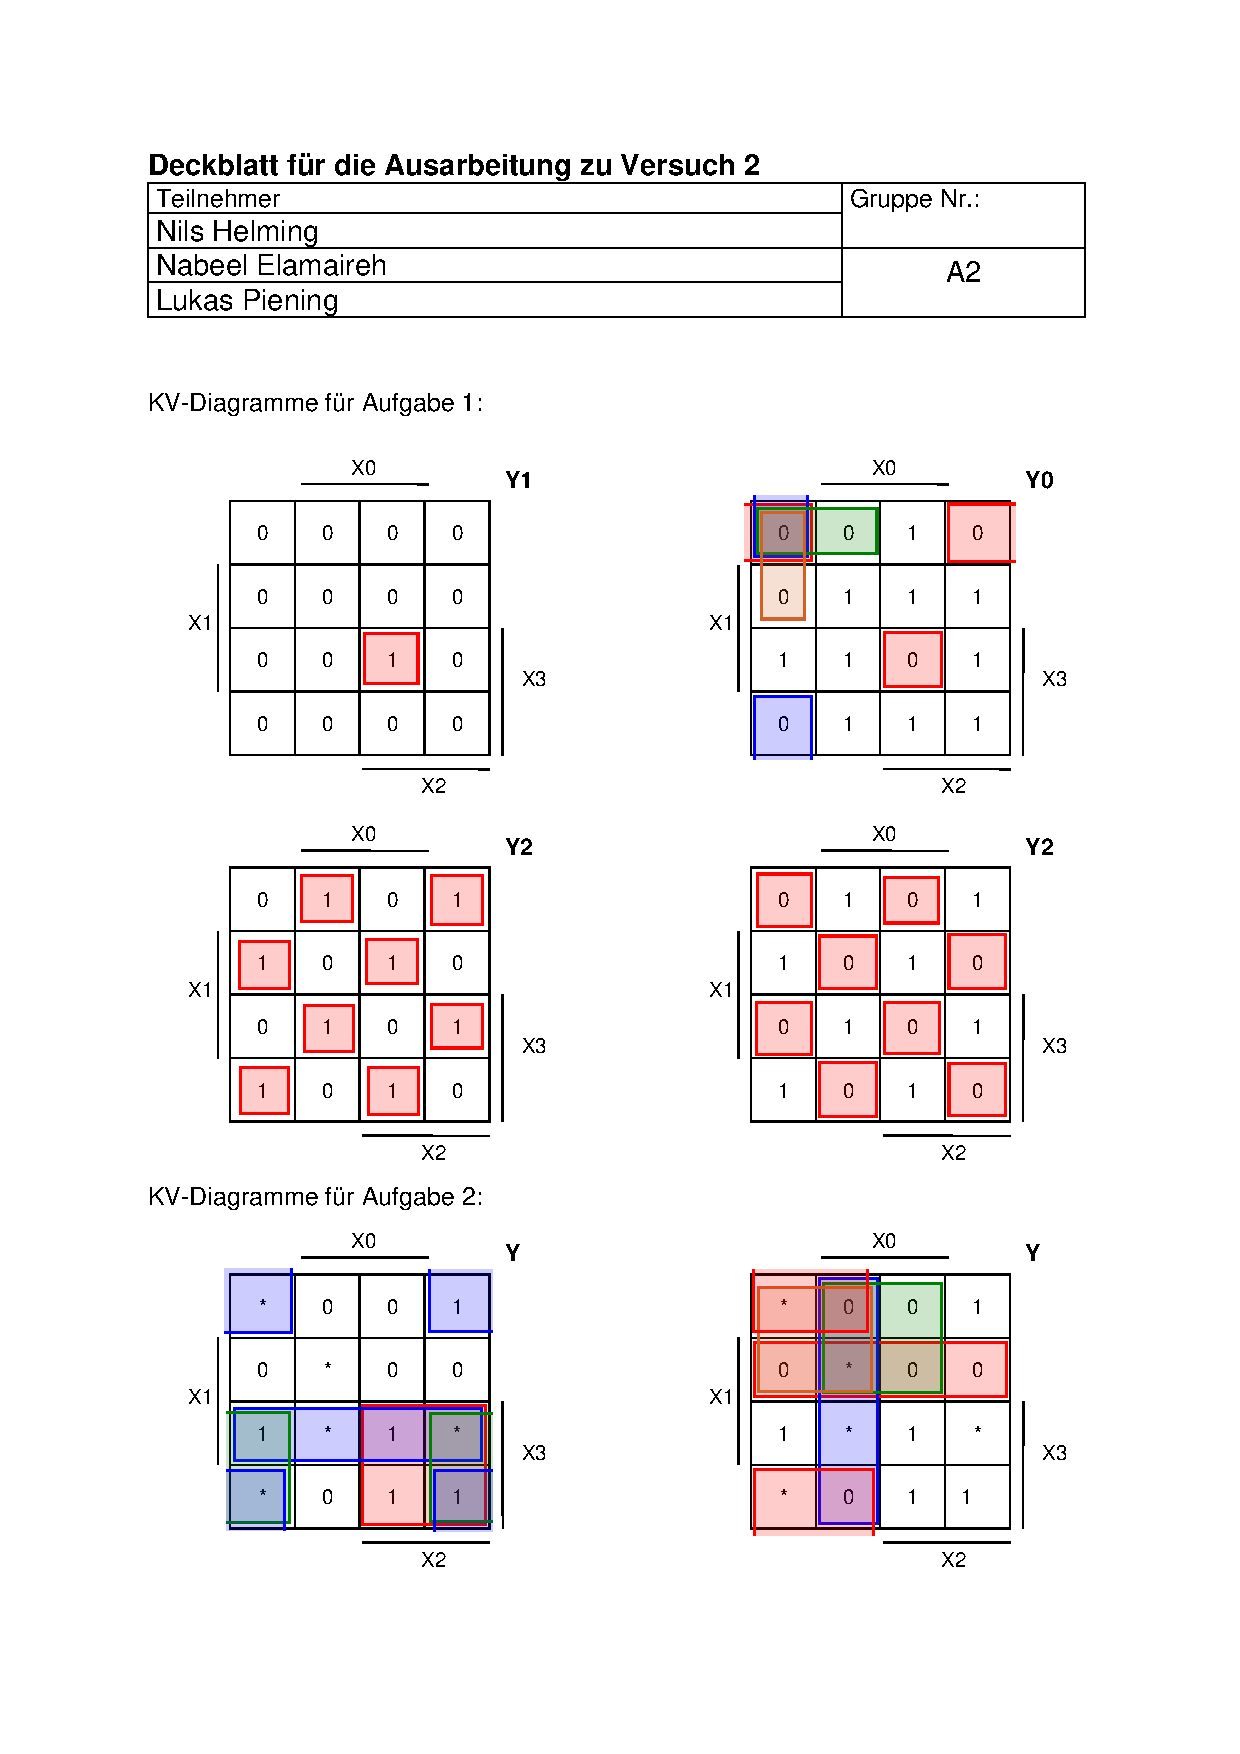
\includepdf[pages=-]{Versuch2H_Deckblatt.pdf}
\section*{Aufgabe 1:}
\subsection*{$Y_1$:}
	\begin{align*}
		Y = (X_3 \A X_2 \A X_1 \A X_0)
	\end{align*}
\subsection*{$Y_0$:}
	\begin{align*}
		\T{Y} &= (X_3 \A X_2 \A X_1 \A X_0) \V (\T{X_3} \A \T{X_1} \A \T{X_0}) \V (\T{X_2} \A \T{X_1} \A \T{X_0}) \V (\T{X_3} \A \T{X_2} \A \T{X_0}) \V (\T{X_3} \A \T{X_2} \A \T{X_1})\\
		&\text{nach dem Shannonschen Gesetz:}\\
		Y &= (\T{X_3} \V \T{X_2} \V \T{X_1} \V \T{X_0}) \A (X_3 \V X_1 \V X_0) \A (X_2 \V X_1 \V X_0) \A (X_3 \V X_2 \V X_0) \A (X_3 \V X_2 \V X_1)
	\end{align*}
\subsection*{$Y_2$:}
	Disjunktive Minimalform:
	\begin{align*}
		Y &= (X_0 \A \T{X_1} \A \T{X_2} \A \T{X_3})\\
			&\V (\T{X_0} \A X_1 \A \T{X_2} \A \T{X_3})\\
			&\V (\T{X_0} \A \T{X_1} \A X_2 \A \T{X_3})\\
			&\V (\T{X_0} \A \T{X_1} \A \T{X_2} \A X_3)\\
			&\V (\T{X_0} \A X_1 \A X_2 \A X_3)\\
			&\V (X_0 \A \T{X_1} \A X_2 \A X_3)\\
			&\V (X_0 \A X_1 \A \T{X_2} \A X_3)\\
			&\V (X_0 \A X_1 \A X_2 \A \T{X_3})\\
	\end{align*}
	Konjunktive Minimalform:
	\begin{align*}
		\T{Y} &= (\T{X_0} \A \T{X_1} \A \T{X_2} \A \T{X_3}) \V (X_0 \A X_1 \A X_2 \A X_3)\\
		 	&\V (X_0 \A X_1 \A \T{X_2} \A \T{X_3}) \V (\T{X_0} \A \T{X_1} \A X_2 \A X_3)\\
		 	&\V (X_0 \A \T{X_1} \A X_2 \A \T{X_3}) \V (\T{X_0} \A X_1 \A \T{X_2} \A X_3)\\
			 &\V (X_0 \A \T{X_1} \A \T{X_2} \A X_3) \V (\T{X_0} \A X_1 \A X_2 \A \T{X_3})\\
			&\text{nach dem Shannonschen Gesetz:} \\
		Y &= (X_0 \V X_1 \V X_2 \V X_3) \A (\T{X_0} \V \T{X_1} \V \T{X_2} \V \T{X_3})\\
		&\A (\T{X_0} \V \T{X_1} \V X_2 \V X_3) \A (X_0 \V X_1 \V \T{X_2} \V \T{X_3})\\
		&\A (\T{X_0} \V X_1 \V \T{X_2} \V X_3) \A (X_0 \V \T{X_1} \V X_2 \V \T{X_3})\\
		&\A (\T{X_0} \V X_1 \V X_2 \V \T{X_3}) \A (X_0 \V \T{X_1} \V \T{X_2} \V X_3)\\
	\end{align*}
	Beide Minimalformen besitzen beide einen Aufwand von $40$.


\section*{Aufgabe 2:}
\subsection*{a)}
	Disjunktive Minimalform:
	\begin{align*}
		Y = (X_3 \A X_2) \V (\T{X_0} \A \T{X_1}) \V (X_3 \A \T{X_0})
	\end{align*}

	Konjunktive Minimalform:
	\begin{align*}
		&& \T{Y} &= (X_1 \A \T{X_3}) \V (X_0 \A \T{X_3}) \V (X_0 \A \T{X_2}) &&\\
		\text{nach dem Shannonschen Gesetz:}&& Y &= (\T{X_1} \V X_3) \A (\T{X_0} \V X_3) \A (\T{X_0} \V X_2) &&\\
	\end{align*}
\subsection*{b)}
	Zur Umsetzung in ein Schaltgatter mit ausschließlich NAND und Inverter-Gattern müssen die Minimalformen umgestellt werden, sodass auch diese nur NAND und Inverter verwenden:

	Disjunktive Minimalform:
	\begin{align*}
		&&Y &= (X_3 \A X_2) \V (\T{X_0} \A \T{X_1}) \V (X_3 \A \T{X_0})&&\\
		\text{AND doppelt negieren:}&& &= \T{\T{(X_3 \A X_2)}} \V \T{\T{(\T{X_0} \A \T{X_1})}} \V \T{\T{(X_3 \A \T{X_0})}}&&\\
		\text{nach DeMorgan:}&& &= \T{\T{(X_3 \A X_2)} \A \T{(\T{X_0} \A \T{X_1})} \A \T{(X_3 \A \T{X_0})}}&&\\
	\end{align*}
	\begin{center}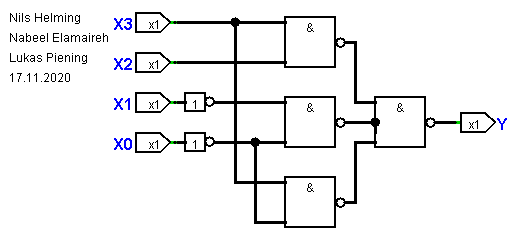
\includegraphics[scale=0.7]{Bilder/DisjunktiveNormalform.png}\end{center}

	\begin{samepage}
	Konjunktive Minimalform:
	\begin{align*}
		&& Y &= (\T{X_1} \V X_3) \A (\T{X_0} \V X_3) \A (\T{X_0} \V X_2) &&\\
		\text{alle nicht negierten Eingänge doppelt negieren:}&& &= (\T{X_1} \V \T{\T{X_3}}) \A (\T{X_0} \V \T{\T{X_3}}) \A (\T{X_0} \V \T{\T{X_2}}) &&\\
		\text{DeMorgan anwenden:}&& &= \T{(X_1 \A \T{X_3})} \A \T{(X_0 \A \T{X_3})} \A \T{(X_0 \A \T{X_2})} &&\\
		\text{gesamten Term doppelt negieren:}&& &= \T{\T{\T{(X_1 \A \T{X_3})} \A \T{(X_0 \A \T{X_3})} \A \T{(X_0 \A \T{X_2})}}} &&\\
	\end{align*}
	\begin{center}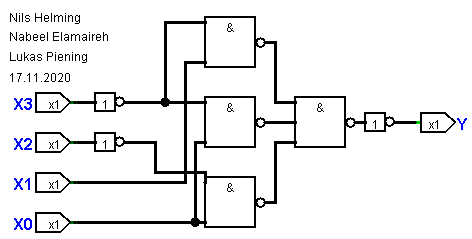
\includegraphics[scale=0.7]{Bilder/KonjunktiveNormalform.png}\end{center}
	\end{samepage}
\end{document}